\chapter{Algorithm Performance with Common Formulas}
To show how our algorithm differs with the current accepted algorithm, we illustrate examples using the FTS in figure \ref{fig:ftsEx}

\begin{figure}
\centering
\begin{tikzpicture}[->,>=stealth',shorten >=1pt,auto,node distance=3.5cm,
                    semithick]
  \tikzstyle{every state}=[fill=red,draw=black,text=black]

  \node[initial,state] (A)                    {$\pi_1$};
  \node[state]         (B) [ right of=A] {$\pi_2$};
  \node[state]         (C) [below of=A] {$\pi_3$};
  \node[state]         (D) [right of=C] {$\pi_4$};
  \node[state]         (E) [right of=B] {$\pi_5$};

  \path (A) edge     [bend left]         node {right} (B)
  		(B) edge     [bend left]         node {left} (A)
		(A) edge     [bend left]         node {down} (C)
  		(C) edge     [bend left]         node {up} (A)
  		(C) edge     [bend left]         node {right} (D)
  		(D) edge     [bend left]         node {left} (C)
  		(B) edge     [bend left]         node {down} (D)
  		(D) edge     [bend left]         node {up} (B)
  		(B) edge     [bend left]         node {right} (E)
  		(E) edge     [bend left]         node {left} (B)
        (A) edge [loop above] node {stay} (A)
        (B) edge [loop above] node {stay} (B)
        (C) edge [loop left] node {stay} (C)
        (D) edge [loop right] node {stay} (D)
        (E) edge [loop above] node {stay} (E);
\end{tikzpicture}
\caption{Simple Finite Transition System}
\label{fig:ftsEx}
\end{figure}
For the simple finite transition system, the set of states $\Pi $ is $ \{\pi_1, \pi_2, \pi_3, \pi_4, \pi_5 \}$, we have the following transitions 
\begin{align*}
\pi_1 \rightarrow_D \pi_1, \hspace{.5cm} & \pi_1 \rightarrow_D \pi_2, \hspace{.5cm}  \pi_1 \rightarrow_D \pi_3 &\\
\pi_3 \rightarrow_D \pi_1, \hspace{.5cm} & \pi_3 \rightarrow_D \pi_3, \hspace{.5cm}  \pi_3 \rightarrow_D \pi_4 &\\
\pi_4 \rightarrow_D \pi_2, \hspace{.5cm} & \pi_4 \rightarrow_D \pi_3, \hspace{.5cm}  \pi_4 \rightarrow_D \pi_4 &\\
\pi_2 \rightarrow_D \pi_1, \hspace{.5cm} & \pi_2 \rightarrow_D \pi_2, \hspace{.5cm}  \pi_2 \rightarrow_D \pi_4 &\\
\pi_2 \rightarrow_D \pi_5, \hspace{.5cm} & \pi_5 \rightarrow_D \pi_2, \hspace{.5cm}  \pi_5 \rightarrow_D \pi_5 &
\end{align*}
the initial state $\Pi_0$ is $\pi_1$, the set of atomic propositions is AP$=\{\pi_1,\pi_2,\pi_3,\pi_4,\pi_5\}$, and the labelling function is defined as $L_D(\pi_i) = \pi_i$ for $i=1,2,\dots,5$. We will treat this as a WFTS. The weights are approximated as the distance between the centers of two states in which a transition exists between. All the states are squares, thus this distance is the same for all transitions. We therefore let the weights be 1 for every transition and 0 to stay in the same state i.e.\ $W_D(\pi_i, \pi_j) = 1$ for $i \neq j$ and $W_D(\pi_i,\pi_i)=0$ for $i=1,2,\dots,5$.

%(\Pi, \rightarrow_D, \Pi_0, AP,L_D)
This FTS will be used in figures unless otherwise stated. We chose it to be very simple because the state explosion problem applies even to the small examples in this report. If we chose a more complex FTS we would not be able to include illustrations of the product automaton because it gets very big very quickly. We will henceforth refer to this FTS as simple FTS. When providing computational results, we will use an FTS that is much larger, to bring out the difference between our algorithm and the accepted algorithm.


\section{Reachability while avoiding regions} 
Reachability while avoiding regions is a property in which we wish to not cross over certain areas, say $\pi_1, \pi_2, \dots, \pi_n$, until we get to a specified region, say $\pi_{n+1}$. After reaching $\pi_{n+1}$ we are free to do what we want. This behaviour is expressed by the formula $\neg (\pi_1 \lor \pi_2 \lor \dots \pi_n) \U \pi_{n+1}$. 

The B\"{u}chi automaton corresponding to this formula is given in figure \ref{fig:ReachAvoid}.

\begin{figure}
\centering
\begin{tikzpicture}[->,>=stealth',shorten >=1pt,auto,node distance=3.2cm,
                    semithick]
  \tikzstyle{every state}=[fill=red,draw=black,text=black]

  \node[initial,state] (A)                    {$q_1$};
  \node[state,accepting]         (B) [right of=A] {$q_2$};

  \path (A) edge              node {$\pi_{n+1}$} (B)
  		(A) edge [loop above] node {$\neg \pi_1 \wedge \neg \pi_2 \wedge \dots \wedge \neg \pi_{n+1}$} (A)
  		(B) edge [loop above] node {$1$} (B);
\end{tikzpicture}
\caption{B\"{u}chi automaton corresponding to $\neg (\pi_1 \lor \pi_2 \lor \dots \lor \pi_n) \U \pi_{n+1}$}
\label{fig:ReachAvoid}
\end{figure}

As we can see $d_p(q_1)=1$ and $d_p(q_2)=0$. For our example, we will look at the specific formula $\neg \pi_4 \U \pi_5$ The product automaton is shown in figure \ref{fig:reachAvoidProduct}

\begin{figure*}
\centering
\begin{tikzpicture}[->,>=stealth',shorten >=1pt,auto,node distance=2.6cm,
                    semithick]
  \tikzstyle{every state}=[fill=red,draw=black,text=black]

  \node[initial,state] (A)                    {$(\pi_1,q_1)$};
  \node[state]         (B) [ right of=A] {$(\pi_2,q_1)$};
  \node[state]         (C) [right of=B] {$(\pi_3,q_1)$};
  \node[state]         (D) [right of=C] {$(\pi_4,q_1)$};
  \node[state]         (E) [right of=D] {$(\pi_5,q_1)$};
  
  \node[state,accepting] 		   (AA)  [below of=A]  {$(\pi_1,q_2)$};
  \node[state,accepting]         (BB) [ right of=AA] {$(\pi_2,q_2)$};
  \node[state,accepting]         (CC) [right of=BB] {$(\pi_3,q_2)$};
  \node[state,accepting]         (DD) [right of=CC] {$(\pi_4,q_2)$};
  \node[state,accepting]         (EE) [right of=DD] {$(\pi_5,q_2)$};  

  \path (A) edge     [bend left]          (B)
        (B) edge     [bend left]          (A)
        (A) edge     [bend left]         (C)
        (C) edge     [bend left]          (A)
        %(C) edge     [bend left]          (D)
        %(D) edge     [bend left]          (C)
		%(B) edge     [bend left]          (D)
        %(D) edge     [bend left]          (B)
        (B) edge               (EE)
        (DD) edge       [bend left]        (BB)
        (BB) edge        [bend left]       (DD)
        (BB) edge        [bend left]       (AA)
        (AA) edge        [bend left]       (BB)
        (BB) edge        [bend left]       (EE)
        (EE) edge        [bend left]       (BB)
        (DD) edge       [bend left]        (CC)
        (CC) edge        [bend left]       (DD)
        (CC) edge        [bend left]       (DD)
        (DD) edge        [bend left]       (CC)
        (CC) edge        [bend left]       (AA)
        (AA) edge        [bend left]       (CC)
        (A) edge [loop above]  (A)
        (B) edge [loop above]  (B)
        (C) edge [loop above]   (C)
        %(D) edge [loop above]   (D)
        (AA) edge [loop below]  (AA)
        (BB) edge [loop below]  (BB)
        (CC) edge [loop below]  (CC)
        (DD) edge [loop below]   (DD)
        (EE) edge [loop below]   (EE);
\end{tikzpicture}
\caption{Product Automaton for $\neg \pi_4 \U \pi_5$ with Simple FTS}
\label{fig:reachAvoidProduct}
\end{figure*}
Note: in figure \ref{fig:reachAvoidProduct} all nodes have a self loop, which are not included for the sake of the reader.
Our algorithm does $n+1$ Dijkstra searches where $n$ is the maximum level of a state in the B\"{u}chi automaton. As we can see in figure \ref{fig:ReachAvoid}, which is the B\"{u}chi automaton corresponding to the general form of reachability while avoiding regions, $n$ is 1 for all formulas of this form. Therefore our algorithm does one Dijkstra search starting from $(\pi_1,q_1)$ which ends at $(\pi_5,q_2)$. This is exactly what the accepted algorithm does, so we do not gain anything when using our algorithm to find an accepting node. However, we do gain a slightly faster run time because we do not have to do a Dijkstra search for every accepting node. We simply do one, and because there $q_2$ in automaton \ref{fig:reachAvoidProduct} has a self loop and every region in the simple FTS has a self loop, every accepting state in the product automaton will have a self loop.

The search of a loop from every accepting node back to itself requires time. We can illustrate this in an example. We have a workspace partitioned into $25 \times 25 = 625$ equally sized squares



The output from the accepted algorithm is

\begingroup
\fontsize{9pt}{12pt}\selectfont
\begin{lstlisting}
Accepted Algorithm
==================
Dijkstra_plan_networkX done within 0.02s: precost 37.00, sufcost 0.00
------------------------------
the prefix of plan **states**:
[((0, 0, 1), 'None'), ((1, 0, 1), 'None'), ((2, 0, 1), 'None'), ((3, 0, 1), 'None'), ((3, 1, 1), 'None'), ((4, 1, 1), 'None'), ((4, 2, 1), 'None'), ((5, 2, 1), 'None'), ((6, 2, 1), 'None'), ((6, 3, 1), 'None'), ((6, 4, 1), 'None'), ((7, 4, 1), 'None'), ((7, 5, 1), 'None'), ((8, 5, 1), 'None'), ((9, 5, 1), 'None'), ((9, 6, 1), 'None'), ((9, 7, 1), 'None'), ((9, 8, 1), 'None'), ((10, 8, 1), 'None'), ((10, 9, 1), 'None'), ((10, 10, 1), 'None'), ((11, 10, 1), 'None'), ((12, 10, 1), 'None'), ((13, 10, 1), 'None'), ((14, 10, 1), 'None'), ((14, 11, 1), 'None'), ((15, 11, 1), 'None'), ((16, 11, 1), 'None'), ((17, 11, 1), 'None'), ((18, 11, 1), 'None'), ((19, 11, 1), 'None'), ((19, 12, 1), 'None'), ((20, 12, 1), 'None'), ((20, 13, 1), 'None'), ((20, 14, 1), 'None'), ((20, 15, 1), 'None'), ((20, 16, 1), 'None')]
the suffix of plan **states**:
[((20, 17, 1), 'None'), ((20, 17, 1), 'None')]
------------------------------
the prefix of plan **actions**:
[(0, 0, 1), (1, 0, 1), (2, 0, 1), (3, 0, 1), (3, 1, 1), (4, 1, 1), (4, 2, 1), (5, 2, 1), (6, 2, 1), (6, 3, 1), (6, 4, 1), (7, 4, 1), (7, 5, 1), (8, 5, 1), (9, 5, 1), (9, 6, 1), (9, 7, 1), (9, 8, 1), (10, 8, 1), (10, 9, 1), (10, 10, 1), (11, 10, 1), (12, 10, 1), (13, 10, 1), (14, 10, 1), (14, 11, 1), (15, 11, 1), (16, 11, 1), (17, 11, 1), (18, 11, 1), (19, 11, 1), (19, 12, 1), (20, 12, 1), (20, 13, 1), (20, 14, 1), (20, 15, 1), (20, 16, 1), (20, 17, 1)]
the suffix of plan **actions**:
['None', 'None']
full construction and synthesis done within 0.11s
\end{lstlisting}
\endgroup

At the top of the output the time taken to calculate the path, the cost of the prefix and the cost of the suffix is given. The states can be thought of as the result of the labelling function, and actions can be thought of the labels of the transition of the B\"uchi automaton. The time for \texttt{full construction and synthesis} is larger than the first time given because it includes the time taken to initialize and construct the graph. This almost always takes the majority of time. For the rest of this report, the calculated paths will appear in the appendix for the ease of the reader.

The output of our algorithm is as follows
\begingroup
\fontsize{9pt}{12pt}\selectfont
\begin{lstlisting}
Our Algorithm
==================
new_algorithm_plan done within 0.01s: precost 37.00, sufcost 0.00
...
full construction and synthesis done within 0.32s 
\end{lstlisting}
\endgroup

As we can see, our algorithm computed the same path in about the same time.%seconds. This may seem weird because we have shown that our algorithm does the same calculation when finding a path from the initial node to an accepting node. The difference is that for each accepting node, a Dijkstra search is performed. In this example, there are 625 accepting states (the number of states in the FTS times the number of states in the B\"uchi automaton). The function \texttt{dijkstra\_predecessor\_and\_distance} from \cite{schult08} is used to calculate the shortest path back to an accepting node. 
\section{Sequencing}
This behaviour is ideal for our algorithm. Sequencing is the behaviour of visiting regions $\pi_1,\pi_2,\dots,\pi_n$ in that order. A formula in this subset of formulas is $\diamond (\pi_3 \land  \diamond \pi_5)$ and is shown in figure \ref{fig:seq}. We note that this automaton is only applicable because of the partition we defined earlier in Definition \ref{def:PM} which makes it impossible for $\pi_i$ and $\pi_j$ to be true at the same time if $i\neq j$. The LTL2BA tool \cite{ltlbuchiwebsite} that is used the github repository \cite{pMasGit} actually generates an automaton with connecting every node. For example, there is an edge from $q_1$ to $q_3$ labelled $\pi_3 \&\& \pi_5 $. This transition is impossible so we take it out before calculating the distances. Our algorithm would not work very well if every state in the B\"uchi automaton had a distance of 1 and the accepting states had a distance of 0.


\begin{figure}
\centering
\begin{tikzpicture}[->,>=stealth',shorten >=1pt,auto,node distance=2.8cm,
                    semithick]
  \tikzstyle{every state}=[fill=red,draw=black,text=black]

  \node[initial,state] (A)                    {$q_1$};
  %\node[state] (B)                    [right of=A]{$q_2$};
  \node[state] (B)                    [right of=A]{$q_2$};
  \node[state,accepting]         (C) [right of=B] {$q_3$};

  \path (A) edge              node {$\pi_{3}$} (B)
  		(A) edge [loop above] node {$\neg \pi_3$} (A)
  		(B) edge [loop above] node {$\neg \pi_5$} (B)
  		(B) edge              node {$\pi_{5}$} (C)
  		(C) edge [loop above] node {$1$} (C);
%  		(C) edge              node {$\pi_{3}$} (D)
 % 		(D) edge [loop above] node {$1$} (D);
\end{tikzpicture}
\caption{B\"uchi Automaton Corresponding to $  \diamond(\pi_3 \land \diamond \pi_5)$}
\label{fig:seq}
\end{figure}

We show why sequencing formulas are ideal for our algorithm in an example using the formula $\diamond (\pi_3 \wedge \diamond \pi_5)$ the simple FTS as before. The product automaton is shown in figure \ref{fig:Sequencing}
\begin{figure*}
\centering
\begin{tikzpicture}[->,>=stealth',shorten >=1pt,auto,node distance=2.6cm,
                    semithick]
  \tikzstyle{every state}=[fill=red,draw=black,text=black]

  \node[initial,state] (A)                    {\footnotesize $(\pi_1,q_1)$};
  \node[state]         (B) [ right of=A] {\footnotesize $(\pi_2,q_1)$};
  \node[state]         (C) [right of=B] {\footnotesize $(\pi_3,q_1)$};
  \node[state]         (D) [right of=C] {\footnotesize $(\pi_4,q_1)$};
  \node[state]         (E) [right of=D] {\footnotesize $(\pi_5,q_1)$};
  
  \node[state] 		   (AA)  [below of=A]  {\footnotesize $(\pi_1,q_2)$};
  \node[state]         (BB) [ right of=AA] {\footnotesize $(\pi_2,q_2)$};
  \node[state]         (CC) [right of=BB] {\footnotesize $(\pi_3,q_2)$};
  \node[state]         (DD) [right of=CC] {\footnotesize $(\pi_4,q_2)$};
  \node[state]         (EE) [right of=DD] {\footnotesize $(\pi_5,q_2)$};
  
  \node[state,accepting] 		   (AAA)  [below of=AA]  {\footnotesize $(\pi_1,q_3)$};
  \node[state,accepting]         (BBB) [ right of=AAA] {\footnotesize $(\pi_2,q_3)$};
  \node[state,accepting]         (CCC) [right of=BBB] {\footnotesize $(\pi_3,q_3)$};
  \node[state,accepting]         (DDD) [right of=CCC] {\footnotesize $(\pi_4,q_3)$};
  \node[state,accepting]         (EEE) [right of=DDD] {\footnotesize $(\pi_5,q_3)$};
  

  \path (A) edge     [bend left]          (B)
        (B) edge     [bend left]          (A)
        %(A) edge     [bend left]         (C)
        %(C) edge     [bend left]          (A)
        %(C) edge		[bend left] 		(D)
        %(D) edge 		[bend left]      (C)
        (A) edge               (CC)
        %(BB) edge               (EEE)
        (BB)	edge			[loop above] (BB)
        (AA)	edge			[loop above] (AA)
        (CC)	edge			[loop above] (CC)
        (DD)	edge			[loop above] (DD)
        (A)	edge			[loop above] (A)
        (E)	edge			[loop above] (E)
        (D)	edge			[loop above] (D)
        (AAA)	edge			[loop below] (AAA)
        (BBB)	edge			[loop below] (BBB)
        (CCC)	edge			[loop below] (CCC)
        (DDD)	edge			[loop below] (DDD)
        (EEE)	edge			[loop below] (EEE)
        (D) edge               (CC)
        (B) edge       [bend left]        (E)
        (E) edge       [bend left]        (B)
        (B) edge       [bend left]        (D)
        (D) edge       [bend left]        (B)
        (BB) edge 			(EEE)
%        (EE) edge			[bend left]		(BB)
        (DD) edge       [bend left]        (BB)
        (BB) edge        [bend left]       (DD)
        (BB) edge        [bend left]       (AA)
        (AA) edge        [bend left]       (BB)
        (CC) edge        [bend left]       (AA)
        (AA) edge        [bend left]       (CC)
        (CC) edge        [bend left]       (DD)
        (DD) edge        [bend left]       (CC)
        
        (DDD) edge       [bend left]        (BBB)
        (BBB) edge        [bend left]       (DDD)
        (BBB) edge        [bend left]       (AAA)
        (AAA) edge        [bend left]       (BBB)
        (BBB) edge        [bend left]       (EEE)
        (EEE) edge        [bend left]       (BBB)
        (DDD) edge       [bend left]        (CCC)
        (CCC) edge        [bend left]       (DDD)
        (CCC) edge        [bend left]       (DDD)
        (DDD) edge        [bend left]       (CCC)
        (CCC) edge        [bend left]       (AAA)
        (AAA) edge        [bend left]       (CCC);
\end{tikzpicture}
\caption{Product Automaton for $\diamond (\pi_4 \wedge \diamond \pi_5)$ with Simple FTS}
\label{fig:Sequencing}
\end{figure*}
In both algorithms the search starts at $(\pi_1,q_1)$. In the first step our algorithm looks at the nodes connected to $(\pi_1,q_1)$ i.e.\ $(\pi_2,q_1)$ and $(\pi_3,q_2)$. Our algorithm notices that we are on level 2, and $(\pi_3,q_2)$ is on level 1. Then it finishes this Dijkstra search and starts another Dijkstra search beginning at $(\pi_3,q_2)$. It will then do one step and search $(\pi_1,q_2)$ and $(\pi_4,q_2)$. Then it will do another step and search $(\pi_2,q_2)$. Then in the third step it searches $(\pi_5,q_3)$. It notices $(\pi_5,q_3)$ is an accepting state and finishes the search with the plan being $R_{new} = (\pi_1,q_1)$, $(\pi_3,q_2)$, $(\pi_4,q_2)$,$(\pi_2,q_2)$, $(\pi_5,q_3)$ (It may turn out that the plan returned is actually $R_{new}=(\pi_1,q_1)$, $(\pi_3,q_2)$, $(\pi_4,q_2)$,$(\pi_2,q_2)$, $(\pi_5,q_3)$, but these paths have an equivalent cost and are found out the same time). 

The accepted algorithm will also start at $(\pi_1,q_1)$ and search $(\pi_2,q_1)$ and $(\pi_3,q_2)$ on the first step. In the next step it will search $(\pi_4,q_1)$, $(\pi_5,q_1)$, $(\pi_1,q_2)$,$(\pi_4,q_2)$. Then it searches $(\pi_2,q_2)$ and then in the next step $(\pi_5,q_3)$. It continues because it has to find the shortest path to \textit{all} accepting nodes. So the next step it searches $(\pi_2,q_3)$, then $(\pi_1,q_3)$ and $(\pi_4,q_3)$ and finally $(\pi_3,q_3)$.

The advantage that our algorithm has over the accepted algorithm is that the accepted algorithm will search through more extraneous nodes, for example $(\pi_5,q_1)$, and that it does not have to find the shortest path to all the accepting nodes. This may not seem like a lot in this example, but when we expand to larger problems the difference becomes significant. 

We now define a workspace to use with our problem. Our workspace is a grid, 25 units across and 25 units up, a total of 625 regions. We say our robot can can move horizontally and vertically, however it cannot move diagonally. Additionally we say that the unit cost of going from any adjacent to another region is 1. The initial position is located at $(0,0)$, region $\pi_1$ is located at (2,24), region $\pi_2$ is located at (12,12), and region $\pi_3$ is located at (20,15) . See figure \ref{fig:workspace}

\begin{figure}[!htb]
\centering
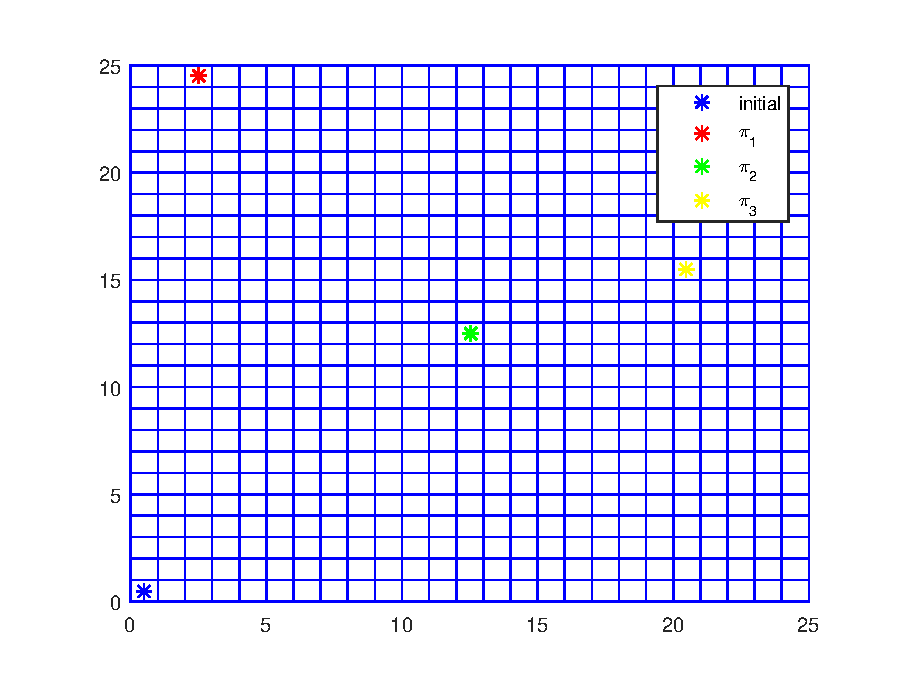
\includegraphics[scale=1]{workspace.eps}
\label{fig:workspace}
\caption{Workspace 1}
\end{figure}

We run both algorithms with the formula of $\diamond (\pi_1 \land \diamond(\pi_2 \land \diamond \pi_3))$. The output from the accepted algorithm is
\begingroup
\fontsize{9pt}{12pt}\selectfont
\begin{lstlisting}
Accepted Algorithm
==================
Dijkstra_plan_networkX done within 0.04s: precost 62.00, sufcost 0.00
...
full construction and synthesis done within 0.19s 
\end{lstlisting}
\endgroup
Our algorithm computed the same path, with an output of

\begin{lstlisting}
Our Algorithm
==================
new_algorithm_plan done within 0.02s: precost 62.00, sufcost 0.00
...
full construction and synthesis done within 0.17s 
\end{lstlisting}
as we can see, the plan synthesis part took half as long; 0.02 seconds compared to 0.04 seconds. We take a look at what causes the increased time. 

\begin{figure}[!htb]
\centering
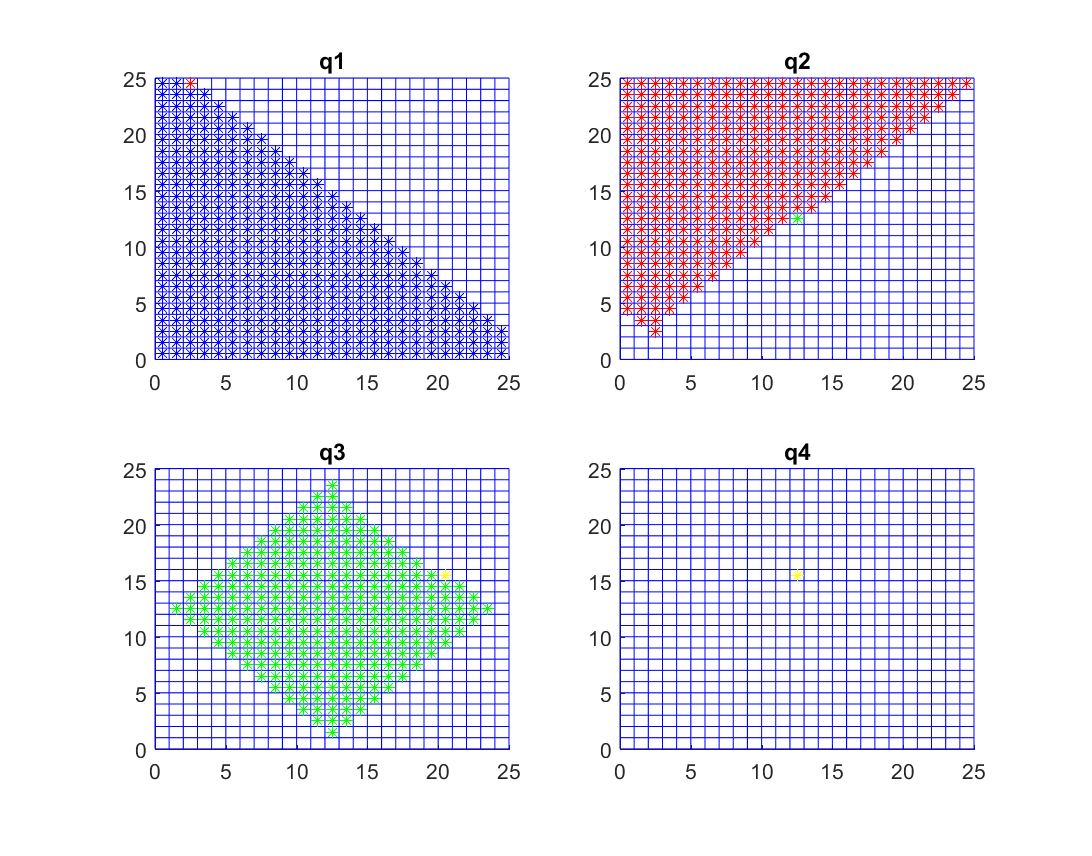
\includegraphics[scale=0.9]{ourPlot}
\label{fig:animOur}
\caption{Nodes searched with our Algorithm}
\end{figure}

\begin{figure}[!htb]
\centering
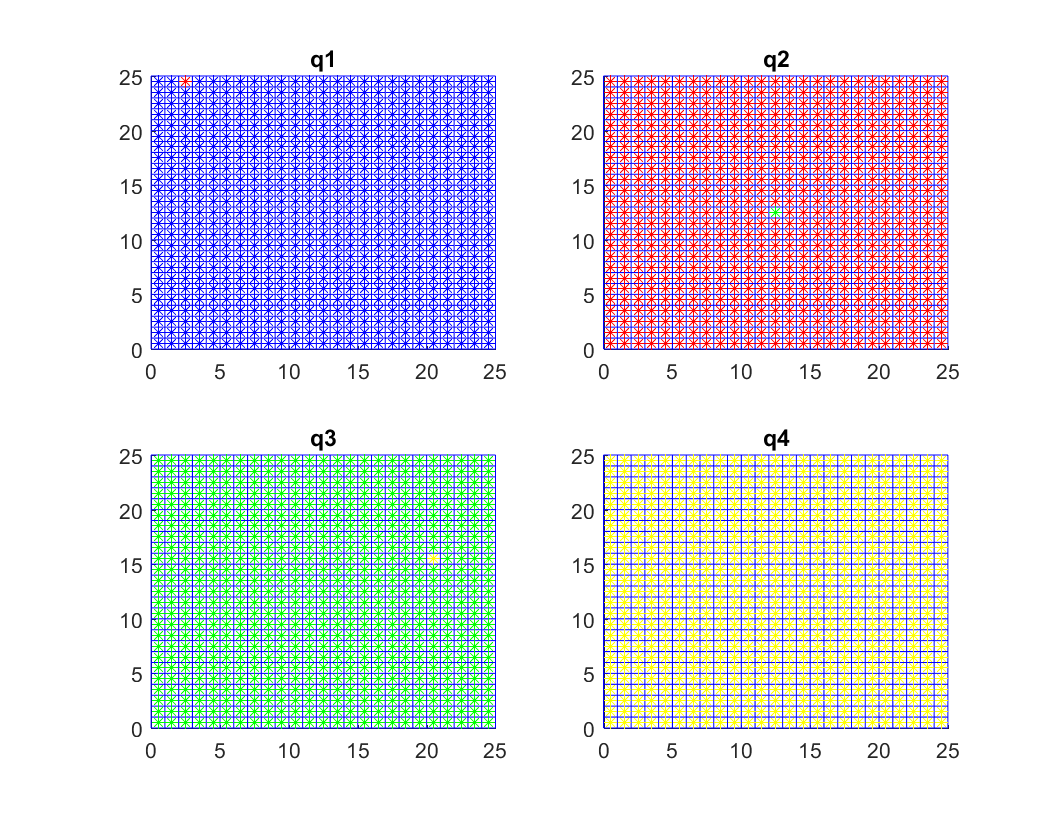
\includegraphics[scale=0.9]{acceptedPlot}
\label{fig:animAccept}
\caption{Nodes searched with the accepted Algorithm}
\end{figure}

Figure \ref{fig:animOur} shows the states searched with our algorithm and figure \ref{fig:animAccept} shows the states visited with the accepted algorithm. Each figure shows a representation of the product automaton. The graph can be thought of as the discretization of the workspace, and there are four corresponding to the four states in the B\"uchi automaton. Any square filled in with blue, red green or yellow has been visited, all others have not. As we can see, our algorithm searches a significantly smaller number of nodes, while the accepted algorithm searches every node.

The FTS has 625 and the B\"uchi automaton has four states, which implies the product automaton has 2500 states. The accepted algorithm computes the shortest paths from the initial node to each of the 2499 other nodes, and then for each of the 625 accepting nodes computes the shortest path back to itself. The algorithm then chooses which combination out of the 625 choices makes the shortest overall run. 

The level of the initial node is three, so our algorithm does three Dijkstra searches; one for each level and one for the accepted node back to itself. To find an accepting node, the the first search searches through 326 nodes, the second 266 nodes, and the third 587 nodes. The last search simply finds the path from the accepting node back to itself, which is a self loop. Thus our algorithm searches 1179 nodes compared to 2500 nodes.  
%Check how many nodes are searched with both algorithms, and show time difference.



\section{Coverage}
A coverage formula represents the statement visit $\pi_1, \pi_2, \dots, \pi_n$ in any order, and is of the form $\varphi = \diamond \pi_1 \wedge \diamond \pi_2 \wedge \dots \wedge \diamond \pi_n$. We show the B\"uchi automaton corresponding to the formula $\diamond \pi_1 \wedge \diamond \pi_2 \wedge \diamond \pi_3$ in figure \ref{fig:buchCov}

\begin{figure}
\centering
\begin{tikzpicture}[->,>=stealth',shorten >=1pt,auto,node distance=3.7cm,
                    semithick]
  \tikzstyle{every state}=[fill=red,draw=black,text=black]

  \node[initial,state] (A)                    {$q_1$};
  \node[state] (C)                    [below of=A]{$q_3$};
  \node[state] (D)                    [right of=C]{$q_4$};
  \node[state]         (B) [left of=C] {$q_2$};
  \node[state] (E) 					[below of=B]{$q_5$};
   \node[state] (F) 					[below of=C]{$q_6$};
   \node[state] (G) 					[below of=D]{$q_7$};
   \node[accepting,state] (H) 					[below of=F]{$q_8$};
  

  \path (A) edge              node {$\pi_{1}$} (B)
   (A) edge              node {$\pi_{2}$} (C)
   (A) edge              node {$\pi_{3}$} (D)
   (B) edge              node {$\pi_{2}$} (E)
   (B) edge              node [near start] {$\pi_{3}$} (F)
   (C) edge              node [near end] {$\pi_{1}$} (E)
   (E) edge              node {$\pi_{3}$} (H)
   (F) edge              node {$\pi_{2}$} (H)
   (G) edge              node {$\pi_{1}$} (H)
   (D) edge              node {$\pi_{2}$} (G)
   (A) edge      [loop above]        node {$\neg (\pi_1 \lor \pi_{2} \lor\pi_3)$} (A)
   (B) edge      [loop left]        node {$\neg (\pi_{2} \lor \pi_3)$} (B)
   (C) edge      [loop below]        node {$\neg( \pi_1 \lor \pi_3)$} (C)
   (D) edge      [loop right]        node {$\neg (\pi_1 \lor \pi_{2}) $} (A)
   (E) edge      [loop left]        node {$\neg  \pi_3$} (E)
   (F) edge      [loop above]        node {$\neg  \pi_2$} (F)
   (G) edge      [loop right]        node {$\neg  \pi_1$} (G)
   (H) edge      [loop below]        node {$1$} (H)
   (D) edge              node [near start] {$\pi_{1}$} (F)
   (C) edge              node [near start] {$\pi_{3}$} (G);
\end{tikzpicture}
\caption{B\"uchi Automaton Corresponding to $\diamond \pi_1 \wedge \diamond \pi_2 \wedge \diamond \pi_3$}
\label{fig:buchCov}
\end{figure}

So, we can see that to get to the accepting node, we have to choose which node to go to first, and which node to go to second (the third node we then have to visit is already decided). So, there are 6 possible paths to take from the initial node, $q_1$ to accepting state $q_8$. This is true in the product automaton too, if we only consider the option of taking the optimal path between nodes. The order that our algorithm will pick is it will pick first pick $\pi_i$ which is the closest to it. From then, it will pick the next closest $\pi_j$ out of the two that have not been visited yet.



When we use our algorithm on a coverage formula, we may not get the optimal path. We will however get an accepting path, with a bound on the cost of our path in terms of the cost of the optimal path. 

We first show that this path corresponds to the one generated by the nearest neighbour approach to the travelling salesperson problem. Next we provide the bound on the cost of our path based on the worst case ratio of the nearest neighbour tour to the optimal tour given by Rosendrantz, Stearns, and Lewis \cite{rosenkrantz74}. 

\subsection{Travelling Salesperson Problem}
The travelling salesperson problem is stated in layman's terms as finding the shortest path for a salesperson to take such that he passes through a given set of cities and then returns back home at the end. More formally, it can be stated as finding the minimum Hamiltonian circuit with the lowest sum of distances between the nodes (cities). This problem has been studied extensively and "give quote about importance". This problem is NP-hard, and thus many algorithms and heuristics exist for finding an approximate solution. One very simple algorithm to do this is called the nearest neighbour algorithm. It says from the starting city, pick the closest city to be the next stop. From there, pick the next closest city not including the starting city, and so on. If there is a tie in the next closest neighbour, we assume that the next node can be decided arbitrarily. This is exactly what our algorithm does in this situation, the first Dijkstra search finds the closest node, and the we start another search. 

To formulate our problem as a travelling salesman problem we use the idea of a dummy node from Lenstra and Rinnooy Kan's computer wiring example in \cite{lenstra75}. In their example, they are designing a computer interface at the Institute for Nuclear Physical Research in Amsterdam. An interface is made up of several modules, with multiple pins on each module. A given subset of pins has to be interconnnected by wires, and at most two wires can be connected to any pin. For obvious regions, it is desirable to minimize the amount of wire used. They show that this is actually a travelling salesperson problem in disguise. The only difference between this problem and a travelling salesman problem is that in the travelling salesman problem, the salesman must return home at the end. This is not true in this problem. It is also not true in our problem, we only need to pass through $\pi_1$, $\pi_2$ and $\pi_3$, there is no need to return to the starting state after we do this. To formulate this seemingly unrelated problem into a travelling salesperson problem, they set $P$ to be the set of pins to be interconnected, $c_{ij}$ to be the distance between pin $i$ and pin $j$. They then introduce a dummy node $*$ that is a distance 0 from all the other nodes i.e.\ $c_{i*} = c_{*i} = 0$ for all i. Then the corresponding problem is solving the travelling salesperson problem on the set of nodes $N=P \cup \{*\}$. 

For our problem, we set $c_{ij}=d(\pi_i , \pi_j)$, for $i,j=0,1,2,3$ where the initial state is from now on known as $\pi_0$, to be the shortest path our robot can take from $\pi_i$ to $\pi_j$, insuring that the triangle inequality is satisfied for all $i$ and $j$. We must preserve the the triangle inequality for a proof of a worst case scenario bound we will provide later on. We use this same idea as above of adding a dummy node, however to preserve the triangle inequality we cannot have the dummy node be distance 0 from the other nodes. Indeed, if $c_{i*} = c_{*i} = 0 $ the triangle inequality would be violated because $c_{i*} + c_{*j} = 0 \geq c_{ij}$ which would make the cost from getting to any point 0, thus rendering the problem extremely trivial. 

We can represent the relationship between the regions in our graph with the following \textit{complete} subgraph, shown in figure \ref{fig:completeGraph}. A complete graph is an undirected graph in which every pair of vertices is connected by an edge. 
\begin{figure}
\centering
\begin{tikzpicture}[-,>=stealth',shorten >=1pt,auto,node distance=5cm,
                    semithick]
  \tikzstyle{every state}=[fill=red,draw=black,text=black]

  \node[state] (A)                    {$\pi_0$};
  \node[state] (B)                    [right of=A]{$\pi_1$};
  \node[state] (C)                    [below of=A]{$\pi_2$};
  \node[state]         (D) [right of=C] {$\pi_3$};

  \path (A) edge              node {$26$} (B)
  		(A) edge 			 node {$24$} (C)
  		(A) edge              node [near start] {$35$} (D)
  		(B) edge 				node [near start] {$22$} (C)
  		(B) edge              node {$27$} (D)
  		(C) edge				node {$11$} (D);
\end{tikzpicture}
\caption{Complete Graph between Regions of Interest}
\label{fig:completeGraph}
\end{figure}

For the distances, we use the so called \textit{Manhattan distance},\\ i.e.\ $d((x_1,y_1),(x_2,y_2)) = |x_1 - x_2| +| y_1 - y_2|$ because our robot can only move horizontally and vertically, not diagonally. Given the weights between the vertices, we easily see that the path that our algorithm, and the nearest neighbour, will take is shown in figure \ref{fig:pathOnComplete}. The cost of this path is 62.

\begin{figure}
\centering
\begin{tikzpicture}[-,>=stealth',shorten >=1pt,auto,node distance=4cm,
                    semithick]
  \tikzstyle{every state}=[fill=red,draw=black,text=black]

  \node[state] (A)                    {$\pi_0$};
  \node[state] (B)                    [right of=A]{$\pi_1$};
  \node[state] (C)                    [below of=A]{$\pi_2$};
  \node[state]         (D) [right of=C] {$\pi_3$};

  \path (A) edge 			 node {$24$} (C)
  		(B) edge              node {$27$} (D)
  		(C) edge				node {$11$} (D);
\end{tikzpicture}
\caption{Nearest Neighbour Path}
\label{fig:pathOnComplete}
\end{figure}

This is not the optimal path though, which is shown in figure \ref{fig:optcompleteGraph} and has a cost of 59.

\begin{figure}
\centering
\begin{tikzpicture}[-,>=stealth',shorten >=1pt,auto,node distance=4cm,
                    semithick]
  \tikzstyle{every state}=[fill=red,draw=black,text=black]

  \node[state] (A)                    {$\pi_0$};
  \node[state] (B)                    [right of=A]{$\pi_1$};
  \node[state] (C)                    [below of=A]{$\pi_2$};
  \node[state]         (D) [right of=C] {$\pi_3$};

  \path (A) edge              node {$26$} (B)
  		%(A) edge 			 node {$24$} (C)
  		%(A) edge              node {$35$} (D)
  		(B) edge 				node {$22$} (C)
  		%(B) edge              node {$27$} (D)
  		(C) edge				node {$11$} (D);
\end{tikzpicture}
\caption{Optimal Path}
\label{fig:optcompleteGraph}
\end{figure}


Because we have to make sure that the dummy node does not change the order that our algorithm and the nearest neighbour algorithm takes we have to set the distance the dummy node is away from every other node to be $max_{i,j} c_{ij} $ where $c_{ij}$ is the distance between the nodes in the complete subgraph in figure \ref{fig:completeGraph}. In our case, this is 35, the path between $\pi_0$ and $\pi_3$. This insures that the path taken is the same as the accepted neighbour because the dummy node will be the last node to be visited. This is because in the nearest neighbour algorithm, ties are broken arbitrarily. Thus, the only time where it is a possibility that the nearest neighbour algorithm goes to the dummy node i.e.\ when the next nodes are $\max_{i,j} c_{ij}$ from the current node is when and if we are faced with the only choice being take the maximum path $\max_{i,j} c_{i,j}$ to $\pi_j$ or to go to the dummy node, and we can choose to go to $\pi_j$ because the ties can be broken arbitrarily. In any other case, the nearest neighbour path will choose a to go to a node where the cost is $c_{i',j'} < c_{i,j}$. 

We show the new subgraph in figure \ref{fig:completeDummy}

\begin{figure}
\centering
\begin{tikzpicture}[-,>=stealth',shorten >=1pt,auto,node distance=5cm,
                    semithick]
  \tikzstyle{every state}=[fill=red,draw=black,text=black]

  \node[state] (A)                    {$\pi_0$};
  \node[state] (B)                    [right of=A]{$\pi_1$};
  \node[state] (C)                    [below of=A]{$\pi_2$};
  \node[state]         (D) [right of=C] {$\pi_3$};
  \node[state] (E)			[right of = D] {$*$}; 

  \path (A) edge              node {$26$} (B)
  		(A) edge 			 node {$24$} (C)
  		(A) edge              node [near end] {$35$} (D)
  		(B) edge 				node [near end] {$22$} (C)
  		(B) edge              node [near start] {$27$} (D)
  		(C) edge				node {$11$} (D)
  		(E) edge 				node {$35$} (D)
  		(E) edge 				[bend left] node {$35$} (C)
  		(E) edge 				node {$35$} (B)
  		(E) edge 				node [near start] {$35$} (A);
\end{tikzpicture}
\caption{Complete Subgraph with Dummy Node}
\label{fig:completeDummy}
\end{figure}

The path that the nearest neighbour algorithm takes in this situation, the complete Hamiltonian circuit, is given in figure \ref{fig:NearNeigDummy}, which gives a total cost of 132.

\begin{figure}
\centering
\begin{tikzpicture}[-,>=stealth',shorten >=1pt,auto,node distance=4cm,
                    semithick]
  \tikzstyle{every state}=[fill=red,draw=black,text=black]

  \node[state] (A)                    {$\pi_0$};
  \node[state] (B)                    [right of=A]{$\pi_1$};
  \node[state] (C)                    [below of=A]{$\pi_2$};
  \node[state]         (D) [right of=C] {$\pi_3$};
  \node[state] (E)			[right of = D] {$*$}; 

  \path (A) edge 			 node {$24$} (C)
  		%(A) edge              node {$35$} (D)
  		%(B) edge 				node {$22$} (C)
  		(B) edge              node [near start] {$27$} (D)
  		(C) edge				node {$11$} (D)
  		%(E) edge 				node {$35$} (D)
  		%(E) edge 				[bend left] node {$35$} (C)
  		(E) edge 				node {$35$} (B)
  		(E) edge 				node [near start] {$35$} (A);
\end{tikzpicture}
\caption{Nearest Neighbour Path with Dummy Node}
\label{fig:NearNeigDummy}
\end{figure}

We note however that this is not the optimal solution. This optimal solution is shown in 
figure \ref{fig:optDummy} and has a cost of 129.

\begin{figure}
\centering
\begin{tikzpicture}[-,>=stealth',shorten >=1pt,auto,node distance=4cm,
                    semithick]
  \tikzstyle{every state}=[fill=red,draw=black,text=black]

  \node[state] (A)                    {$\pi_0$};
  \node[state] (B)                    [right of=A]{$\pi_1$};
  \node[state] (C)                    [below of=A]{$\pi_2$};
  \node[state]         (D) [right of=C] {$\pi_3$};
  \node[state] (E)			[right of = D] {$*$}; 

  \path (A) edge			node {$26$} (B)
  		%(A) edge 			 node {$24$} (C)
  		%(A) edge              node {$35$} (D)
  		(B) edge 				node {$22$} (C)
  		%(B) edge              node {$27$} (D)
  		(C) edge				node {$11$} (D)
  		(E) edge 				node {$35$} (D)
  		%(E) edge 				[bend left] node {$35$} (C)
  		%(E) edge 				node {$35$} (B)
  		(E) edge 				node {$35$} (A);
\end{tikzpicture}
\caption{Optimal Path with Dummy Node}
\label{fig:optDummy}
\end{figure}


\subsection{Cost Bound}

It has been shown \cite{rosenkrantz74} that for an n-node travelling salesperson problem which satisfies the triangle inequality i.e.\ $d(i,j) = d(j,k) \geq d(i,k)$ for all $i,j,$ and $k$ where $d(i,j)$ is the nonnegative distance between nodes $i$ and $j$, 
\begin{align*}
\text{NEARNEIBR} \leq (\frac{1}{2} \lceil \log(n) \rceil + \frac{1}{2})\text{OPTIMAL}
\end{align*}
where NEARNEIBR is the cost of the path generated by the nearest neighbour algorithm and OPTIMAL is the cost of the optimal path. 

Our values do indeed satisfy this inequality
\begin{align*}
\text{NEARNEIBR} &\leq (\frac{1}{2} \lceil \log(n) \rceil + \frac{1}{2})\text{OPTIMAL} \\
132 &\leq (\frac{1}{2} \lceil \log(5) \rceil + \frac{1}{2})129 \\
132 &\leq 258 
\end{align*}
We also see that it is very conservative worst case bound and we will likely do much better.

We provide a proof of
\begin{align}
\dfrac{\text{NEARNEIBR}}{\text{OPTIMAL}} \leq \frac{1}{2} \lceil \log(n) \rceil + \frac{1}{2}
\end{align}
which can be found in \cite{rosenkrantz74}. 
Proof:
We begin by proving 
\begin{align}
\text{OPTIMAL} \geq 2 \sum^{\min(2k,n)}_{i=k+1} l_i \label{eq:showFirst}
\end{align}
for all $k$, $0\leq k \leq n$. 
Let $l_i$ be the length of the $i^{th}$ largest edge in the tour obtained by the nearest neighbour algorithm. For each $i$, $0 \leq i \leq n$, let $a_i$ be the node \textit{onto which} the $i^{th}$ largest edge is added to (that would be the edge with length $l_i$). Let $H$ be the complete subgraph defined on the set of nodes $\{a_i | 1 \leq i \leq min(2k,n)\}$.

Now, let $T$ be the tour in $H$ which visits the nodes of $H$ in the same order as these nodes are visited in an optimal tour of the original graph. Let LENGTH be the length of $T$. We have 
\begin{align}
\text{OPTIMAL $\geq$ LENGTH} \label{eq:optglen}
\end{align}
This is because the tour with cost OPTIMAL passes through all the nodes that the tour with cost LENGTH passes through, and more. Thus if H has an edge $(b,c)$, then the OPTIMAL tour will either have the edge $(b,c)$ or take a less direct route through some of its extra nodes. So the triangle inequality implies (\ref{eq:optglen}).  
   
Let $(a_i,a_j)$ be an edge of $T$. If the nearest neighbour method adds point $a_i$ before $a_j$, we have $d(a_i,a_j) \geq l_i$, where $d(a_i,a_j)$ is the distance between nodes $a_i$ and $a_j$. We also see that if $a_j$ is added first we have $d(a_i, a_j) \geq l_j$. This is because, say we added $a_i$ first, we know there is a point $l_i$ away from $a_i$ that the nearest neighbour method makes the path to. This can be $a_j$, because we know $a_j$ has not been added yet or another node. If it is another node $d(a_i, a_j) \geq l_i$ because the nearest neighbour finds the closest node that has not yet been visited, or $d(a_i, a_j) = l_i$ if $a_j$ is added next. 

Since one has to be added before the other, we have 
\begin{align}
d(a_i , a_j) \geq \min(l_i, l_j) \label{ex:oneBefore}
\end{align}

Summing (\ref{ex:oneBefore}) over the edges of $T$, we get
\begin{align}
\text{LENGTH} \geq \sum_{(a_i,a_j) \text{ in } T} \min(l_i,l_j)  \label{eq:lengmin}
\end{align}

If we let $\alpha_i$ be the number of edges $(a_i, a_j)$ in $T$ for which $l_i$ is selected as $\min(l_i, l_j)$ we obtain 

\begin{align}
\sum_{(a_i,a_j) \text{ in } T} \min(l_i, l_j) = \sum_{a_i \text{ in } H} a_i l_i  \label{ex:lowBound}
\end{align}

Because $a_i$ is the endpoint of two edges in $T$, $\alpha \leq 2$. 

Because $T$ has $\min(2k,n)$ edges (one for each node),

\begin{align}
\sum_{a_i \text{ in } H} \alpha_i = \min(2k,n) 
\end{align}

To get a lower bound on (\ref{ex:lowBound}) we assume that $\alpha_i = 2 $ for $k+1 \leq i \leq \min(2k,n)$ and is zero of $i \leq k$. Thus,

\begin{align}
\sum_{a_i \text{ in } H} a_i l_i \geq 2 \sum_{i=k+1}^{\min(2k,n)} l_i \label{eq:alg2}
\end{align}

Combining (\ref{eq:optglen}), (\ref{eq:lengmin}), (\ref{ex:lowBound}), and (\ref{eq:alg2}), we get

\begin{align*}
\text{OPTIMAL} \geq \text{LENGTH} \geq \sum_{(a_i,a_j) \text{ in } T} \min(l_i,l_j) = \sum_{a_i \text{ in } H} a_i l_i \geq 2 \sum_{i=k+1}^{\min(2k,n)} l_i
\end{align*}
thus proving (\ref{eq:showFirst}). 

We now sum (\ref{eq:showFirst}) for all values of $k$ for all values of $k$ equal to powers of two less than or equal to $n$ i.e. $k = 2^{j} \leq n$ for $j = 0, 1, \dots \lceil \log(n) \rceil - 1$. We then get

\begin{align*}
\sum_{j=0}^{\lceil \log(n) \rceil -1} \text{OPTIMAL} \geq \sum_{j=0}^{\lceil \log(n) \rceil - 1} ( 2 \cdot \sum_{i=2^j + 1}^{\min(2^{j+1,n})} l_i )
\end{align*}
We have
\begin{align*}
\sum_{j=0}^{\lceil \log(n) \rceil -1} \text{OPTIMAL} &\geq 2 \cdot \sum_{i=2}^2 l_i + 2 \cdot \sum_{i=3}^4 l_i + 2 \cdot \sum_{i=5}^8 + \sum_{j=3}^{\lceil log(n) \rceil - 1} (2 \cdot \sum_{i = 2^j+1}^{\min(2^{j+1},n)} l_i )\\
& \geq 2 l_2 + 2 l_3 + 2 l_4 \dots +2l_8 + \sum_{j=3}^{\lceil log(n) \rceil - 1} (2 \cdot \sum_{i = 2^j+1}^{\min(2^{j+1},n)} l_i)
\end{align*}

Therefore we can write

\begin{align}
\lceil \log(n) \rceil \cdot \text{OPTIMAL} \geq 2 \sum_{i = 2}^n l_i \label{eq:lognoptt}
\end{align}

Now OPTIMAL must be longer than twice any edge in the graph because it contains two paths between any given pair of points and these paths are , by the triangle  inequality, longer than the distance of the edge connecting the points directly, i.e.\ OPTIMAL $\geq 2 l_i$ for $i = 1,2,\dots, n$. Specifically,
\begin{align}
\text{OPTIMAL} \geq 2 \l_1 \label{eq:optgl1}
\end{align}

Summing (\ref{eq:lognoptt}) and (\ref{eq:optgl1}) we get 
\begin{align*}
(\log(n)+1) \cdot \text{OPTIMAL} \geq 2 \sum_{i=1}^n l_i
\end{align*}
By definition, $\sum_{i=1}^n l_i = \text{NEARNEIBR}$, thus we have 
\begin{align*}
\text{NEARNEIBR} \leq (\frac{1}{2} \lceil \log(n) \rceil + \frac{1}{2}) \text{OPTIMAL}
\end{align*}
\qed 

We have thus shown that when formulating and solving our problem as a travelling salesman problem with a dummy node, we get the same solution as the nearest neighbour search algorithm. This search algorithm then has a bound on the ratio of the resulting path to the optimal path i.e.\ 
\begin{align*}
\frac{\text{NEARNEIBR}}{\text{OPTIMAL}} \leq (\frac{1}{2} \lceil \log(n) \rceil + \frac{1}{2}) 
\end{align*}

We now must remove the dummy node and provide a bound for the true cost that we will get from our search. 

NEARNEIBR and OPTIMAL as above are costs of Hamaltonian circuits. By definition every node in a Hamaltonian circuit is passed through exactly once. Therefore the dummy node will be passed through exactly once, and we have shown that it will be the last node passed through in the NEARNEIBR. In the NEARNEIBR path, because the dummy node is length $\max_{i,j} c_{i,j}$ it will never be the closest next node, unless we are given the choice to go from $\pi_i$ to $\pi_j$ for $i$ and $j$ being the maximum edge cost in the complete subgraph. In this case we can break the tie arbitrarily and choose to go to $\pi_j$ instead of the dummy node. Thus the path found by the nearest neighbour search will be the path found by our our algorithm, and then going to the dummy node for a cost of $\max_{i,j} c_{i,j}$, then from there going to the initial node to for a cost of $\max_{i,j} c_{i,j}$. Therefore the cost of our algorithm, denote ALGOR is 
\begin{align*}
\text{ALGOR = NEARNEIBR - } 2\max_{i,j} c_{i,j} 
\end{align*}

The path OPTIMAL, however is not guaranteed to have the dummy node be the last node visited. The cost of the path which is optimal and requires that the dummy node is the last node visited, is then greater than or equal to OPTIMAL. This is because of the freedom taken away by requiring the dummy node to be visited last, and less freedom in a minimization problem results in a larger value. Let ACCEPT be the cost of the accepted algorithm for path planning. ACCEPT $+ 2\max_{i,j} c_{i,j}$ is then equal to the cost of the optimal travelling salesman solution which requires that the dummy node is the last node visited. This is because we have already established that the accepted algorithm will find the optimal path. Therefore we have
\begin{align*}
\text{ACCEPT} + 2\max_{i,j} c_{i,j} \geq \text{OPTIMAL}
\end{align*}

Plugging into the travelling salesman bound, we get
\begin{align*}
\text{NEARNEIBR} &\leq (\frac{1}{2} \lceil \log(n) \rceil + \frac{1}{2}) \text{OPTIMAL} \\
\text{ALG} + 2\max_{i,j} c_{i,j} &\leq (\frac{1}{2} \lceil \log(n) \rceil + \frac{1}{2}) \text{OPTIMAL} \\
\text{ALG} + 2\max_{i,j} c_{i,j} &\leq (\frac{1}{2} \lceil \log(n) \rceil + \frac{1}{2}) (\text{ACCEPT} + 2 \max_{i,j} c_{i,j}) \\ 
\end{align*} 
%We can see $\frac{1}{2} \lceil \log(n) \rceil + \frac{1}{2} \geq 0$ for all $n \geq 1$. $n$ is the number of nodes so we can see that it is the case $n\geq 1$. We can  


We can check with our previously calculated values for ALG and ACCEPT
\begin{align*}
\text{ALG} + 2\max_{i,j} c_{i,j} &\leq (\frac{1}{2} \lceil \log(n) \rceil + \frac{1}{2}) (\text{ACCEPT} + 2 \max_{i,j} c_{i,j}) \\ 
62 + 2 (35) &\leq (\frac{3}{2} + \frac{1}{2})(59+70) \\
132 &\leq 258
\end{align*}
We can see that this is still a conservative bound, and emphasize that it is the worst case. Usually the algorithm will preform much better.

\subsection{Simulation}
The actual output from the accepted algorithm is 
\begingroup
\fontsize{9pt}{12pt}\selectfont
\begin{lstlisting}
Accepted Algorithm
==================
Dijkstra_plan_networkX done within 0.08s: precost 59.00, sufcost 0.00
...
full construction and synthesis done within 0.43s 
\end{lstlisting}
\endgroup
and our algorithm is 
\begingroup
\fontsize{9pt}{12pt}\selectfont
\begin{lstlisting}
Our Algorithm
==================
new_algorithm_plan done within 0.02s: precost 62.00, sufcost 0.00
...
full construction and synthesis done within 0.38s 
\end{lstlisting}
\endgroup

As we can see our algorithm calculates the path in 0.02 seconds while the accepted algorithm takes 0.08 seconds. We can break down the searches as we did before. 

The accepted algorithm does one Dijkstra search of all 5000 states in the product automaton (625 states in the FTS and eight in the B\"uchi automaton). Even though there are eight states in the B\"uchi automaton, the initial node is still only on level three. Therefore we only do three searches to find an accepting node. The first searches 326, the second 266, and the third 587. Thus our algorithm searches 1179 nodes compared to 5000 by the accepted algorithm and returns a path of cost 62 compared 59.

\section{Recurrence (Liveness)}
Recurrence is coverage over and over again, and can be expressed as $\smallsquare(\diamond \pi_1 \land \diamond \pi_2 \land \dots \land \diamond \pi_n)$. This example is interesting for two reasons: it is prone to B\"{u}chi automata that are not tight \cite{schuppan05}, and an accepting path for it cannot stay in one state (in contrast to the other formulas, in which all accepting states have self loops). We first look at the tightness.

\subsection{Tightness}
A tight B\"uchi automaton is one that accepts the minimum prefix and the minimum suffix. We begin showing that the automaton produced for these formulas by \cite{ltlbuchiwebsite} is not tight. We consider the formula $\smallsquare(\diamond \pi_1 \land \diamond \pi_2 \land \diamond \pi_3)$. The B\"{u}chi automaton corresponding to this formula, as calculated by \cite{gastin01} is given in figure \ref{fig:gasBuchiRec}

\begin{figure}
\centering
\begin{tikzpicture}[->,>=stealth',shorten >=1pt,auto,node distance=2.8cm,
                    semithick]
  \tikzstyle{every state}=[fill=red,draw=black,text=black]

  \node[initial,state] (A)                    {$q_1$};
  \node[state] (B)                    [right of=A]{$q_2$};
  \node[state,accepting] (C)                    [right of=B]{$q_3$};

  \path (A) edge              node {$\pi_{1}$} (B)
  		(A) edge [loop above] node {$\neg \pi_1$} (A)
  		(B) edge [loop above] node {$\neg \pi_2$} (B)
  		(B) edge              node {$\pi_{2}$} (C)
  		(C) edge [bend left=45] node {$\neg \pi_1$} (A)
  		(C) edge  [bend left] node {$\pi_{1}$} (B);
%  		(D) edge [bend right] node {$\neg \pi_1$} (A)
 % 		(D) edge [bend left] node {$\pi_1$} (B);
\end{tikzpicture}
\caption{B\"uchi Automaton for $\smallsquare(\diamond \pi_1 \land \diamond \pi_2 )$ 1}
\label{fig:gasBuchiRec}
\end{figure}
Note: Again, the actual automaton generated has much more edges. %For example, there is an edge from $q_4$ to $q_2$ which is labelled $\pi_1 \&\& \pi_2$. It is impossible for us to make this transition because $\pi_i$ for all $i$ is a region in our partition. This is because the requirements of our partition are chosen specially to guarantee that we are never in two regions at once. Thus they are excluded in the interest of the reader. 
In this automation, $d(q_1)=2$, $d(q_2)=1$, and $d(q_3)=0$. So, to get from $q_{init}' = \langle \pi_2, q_1 \rangle \in Q_0'$, we have to first get down to level 2. Given the B\"{u}chi automaton \ref{fig:gasBuchiRec} the only way to do this is to go to region $\pi_1$.  In this case the same statement holds for $\pi_2$. It follows that the prefix with the least cost is a concatenation of the shortest paths down from each each level (first to $\pi_1$, etc).


This path however is in general not truly optimal. It is because the B\"{u}chi automaton given in figure \ref{fig:gasBuchiRec} not a tight B\"{u}chi automaton \cite{schuppan05}. A B\"{u}chi automaton is tight if it accepts the shortest lasso (prefix and suffix). The loss of this optimality property is due to the fact that the algorithm in \cite{gastin01} simplifies the B\"{u}chi automaton which is usually a good thing because it leads to a lower computational complexity in most applications. We take a look at a different automaton corresponding to the formula $\smallsquare(\diamond \pi_1 \land \diamond \pi_2)$, shown in figure \ref{fig:otherBuchiRec}. 

\begin{figure}
\centering
\begin{tikzpicture}[->,>=stealth',shorten >=1pt,auto,node distance=5cm,
                    semithick]
  \tikzstyle{every state}=[fill=red,draw=black,text=black]

  \node[initial,state] (A)                    {$q_1$};
  \node[state]         (B) [ right of=A] {$q_2$};  
  \node[state] 		   (C)  [below of=A]  {$q_3$};
  \node[state,accepting]       (D) [ right of=C] {$q_4$};

  \path (A) edge         node {$\pi_{1}$}   (B)
        (B) edge       node [swap] {$\pi_{2}$}    (D)
        (A) edge       node [swap] {$\pi_{2}$}  (C)
        (C) edge     node {$\pi_{1}$}       (D)
        (A) edge [loop above] node {$\neg \pi_1 \wedge \neg \pi_2$} (A)
        (B) edge [loop above] node {$\neg \pi_2$} (B)
        (C) edge [loop below] node {$\neg \pi_1$} (C)
        (D) edge [bend left] node {$\pi_2$} (C)
        (D) edge [bend right] node [swap] {$\pi_1$} (B)
        (D) edge node{$\neg \pi_1 \wedge \neg \pi_2$} (A);
\end{tikzpicture}
\caption{B\"uchi Automaton for $\smallsquare(\diamond \pi_1 \land \diamond \pi_2)$ 2}
\label{fig:otherBuchiRec}
\end{figure}

In this automaton, $d(q_1) = 2$, $d(q_2) = d(q_3) = 1$, and $d(q_4)= 0$. So, we are starting at the same level i.e. 2, however this time we have two choices about what to do to get down to level 2; we can go to $\pi_1$ or $\pi_2$. Being able to choose is good in the sense that we can now find the optimal path, and bad in the sense that the extra state in the $B\"{u}chi$ automaton increased the size of the product automaton by 33\% (hence increasing the time it takes to search the automaton). This very well illustrates the trade off between the search time and optimally/cost of the resulting run. We propose that this is a good way to think about our algorithm. There is a trade off that sometimes it will not find the optimal run, even if this is possible, though it will be faster. 

\subsection{Suffix}
The second aspect of this problem that we wish to look at is fact that it does not have a trivial suffix. In the other examples we have looked at, the suffix of the calculated path (with our algorithm and the accepted algorithm) was a single state; that is, the formula could be satisfied by staying in one state indefinitely. In this example, $\pi_1,$ $\pi_2$, and $\pi_3$ must all be visited infinitely often, and thus these states must be in the suffix. 

The applicability of our algorithm to find the suffix has to be considered. For the total run, R, to be accepting, $\Inf(R) \cap \F$ must not be empty. We are specifically looking for runs of the form 
\begin{align*}
R &= \langle R_{pre}, R_{suf} \rangle = q_0 q_1 \dots q_f [q_f q_{f+1} \dots q_n]^\omega
\end{align*}     
where $q_f \in \F$. Thus when calculating to the suffix we must find the path back to the \textit{same} accepting state. We cannot not just look for any accepting state as we do in the prefix calculation. Our algorithm in general only looks for an accepting state, not a specific accepting state. Thus we have to do a Dijkstra search and if there is a path back to the accepting state it will find it. There is a benefit in this though because our algorithm only has to find the shortest path back to one accepting state, not all of them.
%We notice how in figure \ref{fig:gasBuchiRec} there is only one arrow to the accepting state, labelled $\pi_5$. This implies that the only way to get down to level 0 is to go to $\pi_5$, and thus go to the accepting state $\langle \pi_5, q_3 \rangle$. There is no self loop on $q_3$, so we leave $q_3$ immediately. This implies that the only reachable accepting state is $\langle \pi_5, q_3 \rangle$. So because there is only one accepting state, our algorithm will find this state again, and thus is appropriate for finding the suffix. 

%In \ref{fig:otherBuchiRec} on the other hand, there are two arrows going to the accepting state and there is no self loop. This implies that there are two reachable accepting states i.e.\ $\langle \pi_3, q_4 \rangle$ and $\langle \pi_5, q_4 \rangle$. This poses a problem to our algorithm that is only guaranteed to reach an accepting state. We thus propose using Dijkstra's search algorithm to find the path from the accepting node back to itself.   

\subsection{Simulation}





We have shown previously that given the B\"{u}chi automaton by \cite{ltlbuchiwebsite}, prefix with the least cost is a concatenation of the shortest paths down from each each level (first to $\pi_1$, etc). Our algorithm goes to $\pi_1$ where it can get down a level and then starts a new Dijkstra search. Our algorithm does a Dijkstra search at each level so it will return this path as the prefix. The accepted algorithm will also return this prefix. 

The algorithms produced the same path. The accepted algorithm did this in 
\begingroup
\fontsize{9pt}{12pt}\selectfont
\begin{lstlisting}
Accepted Algorithm
==================
Dijkstra_plan_networkX done within 16.17s: precost 62.00, sufcost 60.00
------------------------------
...
full construction and synthesis done within 16.35s 
\end{lstlisting}
\endgroup
while our algorithm did it in
\begingroup
\fontsize{9pt}{12pt}\selectfont
\begin{lstlisting}
Our Algorithm
==================
new_algorithm_plan done within 0.04s: precost 62.00, sufcost 60.00
------------------------------
...
full construction and synthesis done within 0.21s 
\end{lstlisting}
\endgroup
As we can see, this is the greatest difference in times out of all the examples so far. But why? This is the first example when the suffix is not trivial. In our algorithm, again we search 326+266+587 = 1179 nodes to find the first accepting node. We then do a Dijkstra search to find the shortest path back to this accepting node. This search searches 1879 nodes, resulting in a total search of 3058 nodes. The accepted algorithm does a search of 1879 to find the accepting nodes, and then a search from every accepting node back to itself. These searches are not trivial any more, so each of these searches look through either 1879 or 1880 nodes depending on the accepting node. Seeing as there are 625 accepting nodes, this results in searching 1174996 nodes. This is where the difference comes from. 
